%%%%%%%%%%%%%%%%%%%%%%%%%%%%%%%%%%%%%%%%
% PDF compatibility code. 
\makeatletter
\newif\ifpdflatex@
\ifx\pdftexversion\@undefined
\pdflatex@false
%\message{Not using pdf}
\else
\pdflatex@true
%\message{Using pdf}
\fi

\newcommand{\latexorpdf}[2]{
  \ifpdflatex@ #2
  \else #1
  \fi
}

\makeatother

\newcommand{\pformat}{a4paper}

%%%%%%%%%%%%%%%%%%%%%%%%%%%%%%%%%%%%%%%%

\latexorpdf{
\documentclass[\pformat,12pt]{jarticle}
}{
\documentclass[\pformat,pdftex,12pt]{jarticle}
}

\usepackage[dvipdfmx]{graphicx, color}
\usepackage[dvipdfmx,bookmarks=true,bookmarksnumbered=true,colorlinks,plainpages=true]{hyperref}

\usepackage{toolbox}
\usepackage{vdmsl-2e}
\usepackage{makeidx}
\usepackage{alltt}
%\usepackage{graphics}
%\usepackage{verbatim}
\usepackage{ifthen}
\usepackage{verbatimfiles}
%\usepackage{color}
\usepackage{longtable}
%\usepackage{path}
\usepackage{here}

\graphicspath{{figures/}}
\def\seename{$\Rightarrow$}

% Koizumi change start
\ifnum 42146=\euc"A4A2 \AtBeginDvi{\special{pdf:tounicode EUC-UCS2}}\else
\AtBeginDvi{\special{pdf:tounicode 90ms-RKSJ-UCS2}}\fi
% Koizumi change end

\makeindex

% The use of /VDMPP ifdef's have basicly been exchanged with the
% use of LaTeX ifthenelse's.  For this two LaTeX boolean value  and
% VDMpp have been defined  (Lowercase p's are used to avoid conflict with
% the VDMPP environment variable.  The typical use are:
%   \ifthenelse{\boolean{VDMsl}}{vdmsl-text}{vdmpp-text}
%   \ifthenelse{\boolean{VDMsl}}{vdmsl-text}{}
%   \ifthenelse{\boolean{VDMpp}}{vdmpp-text}{}
% The advantage of this as opposed to ifdef's is that within a general
% paragraph specific VDM-SL and VDM++ parts can be distinguished without
% problematic empty lines.
% 
% The values are initialised such that exactly one of the values is true
% and the other is false.  This should hopefully avoid strange behaviour
% due to possible preprossing errors.  The default case is VDM-SL.
\newboolean{VDMsl}
\setboolean{VDMsl}{true}
\newboolean{VDMpp}
\setboolean{VDMpp}{false}
\setboolean{VDMsl}{true}
\setboolean{VDMpp}{false}


\def\vdmsl{{\small VDM-SL}}
\def\vdmpp{{\small VDM}$^{++}$}
\newcommand{\vdmslpp}{VDM-SL}
\newcommand{\vdmslppEm}{VDM-SL}
\newcommand{\ToolboxName}{VDM-SL Toolbox}
\newcommand{\Toolbox}{Toolbox}
\newcommand{\toolbox}{Toolbox}
\newcommand{\vdmde}{vdmde}
\newcommand{\vdmgde}{vdmgde}
\newcommand{\vdmhome}{vdmhome}
\newcommand{\vdmdeNineteen}{vdmde-19}
\newcommand{\vdmdeNineteenEl}{vdmde-19.el}
\newcommand{\VdmSlPp}{\VdmSl}

\newcommand{\guicmd}[1]{{\sf #1}}

\begin{document}
\vdmtoolsmanualscsk{C++コード生成マニュアル(VDM-SL)}{2.0}


\newcommand{\tcg}{コードジェネレータ}
\newcommand{\Tcg}{コードジェネレータ}


\newcommand{\libmancite}{\cite{LibMan-SCSK}}
\newcommand{\langmancite}{\cite{LangMan-SCSK}}
\newcommand{\cg}{VDM-SL to C++ Code Generator}
%\newcommand{\toolbox}{VDM-SL Toolbox}
\newcommand{\MCL}{VDM C++ Library}
\newcommand{\VDM}{VDM-SL}


%Installation should be described in the Installation document.
\section{導入}


\cg\ は、\VDM\ 仕様から C++ コード自動生成を行うための支援をする。
これにより、\tcg\ は \VDM\ 仕様に基づいたアプリケーションの実装を、速い方法で提供する。

 \Tcg\ は \ToolboxName{}に対しアドオン形式をとる。
このインストールについては、文書\ifthenelse{\boolean{VDMsl}}{\cite{InstallMan-SCSK}}{\cite{InstallPPMan-SCSK}}に記載されている。
本書は {\em VDMToolsユーザマニュアル( \VDM{} )}\ifthenelse{\boolean{VDMsl}}{\cite{UserMan-SCSK}}{\cite{UserManPP-SCSK}} の拡張であり、 \cg{}への導入を行う。

コードジェネレータは、 \VDM\ 構成要素全体のおよそ 95\% をサポートする。
補足として、 生成コードの一部を手書きコードに置き換えることがユーザーに許されている。

本書は以下のように構成されている:

第~\ref{invoking}章で、 \VDM\ 仕様が正しい C++ コードを生成するために満たされなければならない要件を並べる。
さらにこの章で、 \ToolboxName{}からC++ ファイルを起動する方法を述べる。
最後に、コード生成された C++ ファイルを記載する。

第~\ref{interfacing}章は、インターフェイスを記述しながら C++ 生成コードへの導入を行い、そしてそれをどのように手書きコードと結び付けるかを説明する。
さらに、 C++ コードのコンパイル、リンク、実行の方法まで説明する。

第~\ref{sec:unsupported}章では、 \tcg{}でサポートされない \VDM\ 構成要素をまとめて示す。

第~\ref{sec:relation}章は、C++ 生成コード構造の詳細を記載する。
加えて \VDM\ とC++ のデータ型間の関連を説明し、 \cg{}の開発中に用いる名称仕様を含めて、設計上決められている事柄をいくつか述べる。
ここは、\tcg\ を職業的に使用する前には集中的に学習すべき章である。


\section{コードジェネレータの起動}\label{invoking}


%Type \path+codegen+
%and the specification is type checked and the files \path+DefaultMod.h+
%and \path+DefaultMod.cc+ are generated (On Windows platforms the
%implementation file is named \path+DefaultMod.cpp+).

%A detailed description of the usage of the \cg{} is given in the
%Sections 4 and 5 in {\em User Manual for the IFAD \VDM{} Toolbox\/}
%\cite{UserMan}.
%#endif 

\tcg\ の使用を始めるため、1つ以上のファイルにわたった\VDM\ 仕様を書いておくべきであろう。
\Toolbox\ の配布中に、様々なソートアルゴリズムの仕様が含まれている。
この仕様は、以下において \tcg{}の使用を記述するために用いられることとなる。 
これは\ifthenelse{\boolean{VDMsl}}{\cite{SortEx-SCSK}}{\cite{SortExpp-SCSK}}で述べられている。
この手順1つ1つを、自身のコンピュータ上で確認していくことが推奨される。
そのため、ディレクトリ\path+vdmhome/examples/sort+ をコピーしそこへ \path+cd+ にて移動すること。

C++ コードを生成する前に、 \VDM\ 仕様が必要な要件を満たしているかどうか確認する必要がある。
この要件は第~\ref{requirements}章に記述されている。
第~\ref{gui} 章と ~\ref{commandline}章では、 \ToolboxName\ を用いてグラフィカルインターフェイスやコマンドラインから C++ コードを生成する方法を説明する。
第~\ref{sec:cppfiles}章では、コード生成された C++ ファイルを記載する。

\subsection{コード生成のための要件}\label{requirements}

 \Tcg\ は、正確なコード生成のために、 \VDM\ 仕様中の全モジュールの構文チェックがなされていることを要求する。

さらに \tcg\ のみ、正しい型のモジュールに対して、コード生成を行うことができる。\footnote{ \langmancite で説明されているように、よく形式化された2つのクラスが存在する。 現内容では、可能な限りよく形式化された型正確性を意味する。} 
コード生成を行う前に、そのモジュールが型チェックされていない場合は、 \Toolbox{}により自動的に型チェックが行われる。 

\subsection{グラフィカルインターフェイスの利用}\label{gui}

ここでは \ToolboxName{}のグラフィカルユーザーインターフェイスから、どのようにソート例題をコード生成するかを述べていく。

\ToolboxName\ は\path+vdmgde+\index{vdmgde!starting}コマンドで始める。 
ソートの例題に相当するコードを生成するには、 \path+/vdmhome/examples/sort+ディレクトリに置かれたすべての\ifthenelse{\boolean{VDMpp}}{すべての {\tt *.rtf} ファイル}{ファイル {\tt  sort.rtf}} を含めて新しいプロジェクトを生成することである。
プロジェクトの構成法の記載としては、 \ifthenelse{\boolean{VDMsl}}{\cite{UserMan-SCSK}}{\cite{UserManPP-SCSK}} を参照のこと。

最初はファイルに対して構文チェックと型チェックを行う必要がある: 手作業で行わない場合には、\tcg\ が起動されるとき Toolbox が自動的にこれを行うはずである。
ソート例題の仕様では、エラーなしで両チェックを通過する。
その後\ifthenelse{\boolean{VDMsl}}{the module {\em DefaultMod}}{すべてのクラス} を選択して、\raisebox{-1.0mm}{
\includegraphics[width=0.03\textwidth]{cplusplus}} (\guicmd{Generate C++}) ボタンを押すことで、 \tcg\ が起動可能となる。
1つ以上のファイルあるいはクラスを選択することができ、この場合にはこれらが C++コードに翻訳される。
この手順の結果が 図~\ref{fig:cg}に示されている。


\begin{figure}[tbh]
\begin{center}
\mbox{}
\resizebox{9cm}{!}{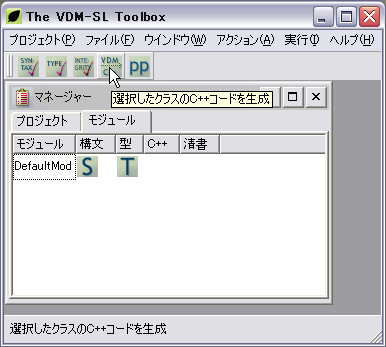
\includegraphics{cgsl1}}
\caption{ソート例題のコード生成}\label{fig:cg}
\end{center}
\end{figure}

仕様中の各 \ifthenelse{\boolean{VDMsl}}{module - in
  this example only one - }{クラス} に対してコードが生成されると、図~\ref{fig:cg2}に見られるようにToolbox は大きな {\em \large{C}}を書き入れてこれを知らせる。
プロジェクトファイルのおかれたディレクトリ中で、たくさんの C++ ファイルが生成される。
プロジェクトファイルの存在しない場合には、これらのファイルは \ToolboxName\ が始められたディレクトリに書かれることになる。

ソート例題に対してコード生成を行う時、\tcg{}によって警告が1つ生成されるため、図~\ref{fig:cg_error}のような {\em Error} ウィンドウが出る。

\begin{figure}[tbh]
\begin{center}
\mbox{}
\resizebox{9.2cm}{!}{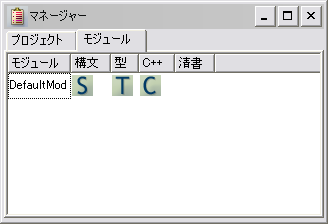
\includegraphics{cgsl2}}
\caption{ソート例題のコード生成}\label{fig:cg2}
\end{center}
\end{figure}


\begin{figure}[tbh]
\begin{center}
\mbox{}
\resizebox{9.2cm}{!}{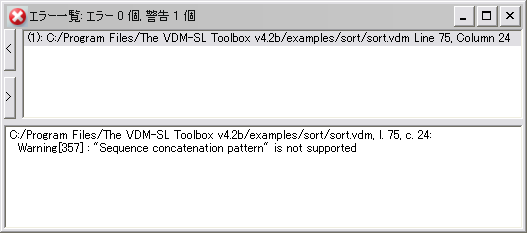
\includegraphics{cgsl3}}
\caption{コードジェネレータで生成された警告}\label{fig:cg_error}
\end{center}
\end{figure}


この警告は、\tcg{}では連結パターンがサポートされないことを示している。
\tcg\ はこの構成要素に対して、実行可能なC++ コード生成を行うことができないということを意味する。
生成されるコードはコンパイル可能なものであるが、サポートされない構成要素が含まれる枝葉部分の実行は実行時エラーを引き起こす。 
第~\ref{sec:unsupported}章で、サポートされない構成要素の詳細リストを提示する。

\tcg\ のユーザーは、実行時エラーの位置情報を含めたコード生成を選択できる。
{\em 出力位置情報} オプションが選択されていると、実行時エラーの原因である \VDM\ 仕様における位置 (ファイル名および行番号と列番号)を実行時エラーメッセージで伝えてくれる。
 図~\ref{fig:option}で示すように、オプションメニューでこの機能は設定できる。

\begin{figure}[tbh]
\begin{center}
\mbox{}
\resizebox{9cm}{!}{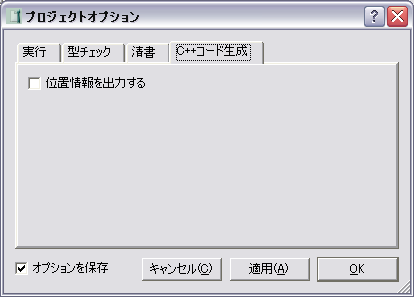
\includegraphics{cgsl4}}
\caption{実行時エラーで生成位置情報に対するオプション}\label{fig:option}
\end{center}
\end{figure}
  
ソート例題に対しては \texttt{MergeSort} 関数の実行が、ここで述べた実行時エラーを引き起こす。
記載したオプション設定を行わなかった場合、相当する C++ コードの実行で次のエラーメッセージが出る:
\begin{quote}
\begin{verbatim}
The construct is not supported: Sequence concatenation pattern
\end{verbatim}
\end{quote}
一方、オプションを設定した場合は次のようなエラーメッセージとなる:
\begin{quote}
\begin{verbatim}
Last recorded position:
In: sort.vdm. At line: 43 column: 18
The construct is not supported: Sequence concatenation pattern
\end{verbatim}
\end{quote}

\subsection{コマンドラインインターフェイスの使用}\label{commandline}

 \ToolboxName\ をコマンドラインから実行する場合にも、もちろん\Tcg\ を起動できる。
これは以下に簡単に述べられている。

\ToolboxName\ は、コマンドラインから {\tt  \vdmde}\index{vdmde!starting}コマンドで始める。コードを生成するために -c オプションを用いる:

\begin{quote}
\begin{verbatim}
vdmde -c [-r] specfile, ...
\end{verbatim}
\end{quote}

ソート例題のコード生成を行うために、次のコマンドを
\path+vdmhome/examples/sort+ ディレクトリで実行する:

\begin{quote}
\begin{verbatim}
vdmde -c sort.vdm
\end{verbatim}
\end{quote}

仕様は最初に構文解析がなされる。
構文エラーが検出されない場合、できる限り適正となるように型チェックがなされる。
型エラーが検出されなかった場合には、仕様は変換され最後にたくさんの C++ ファイルになる。
グラフィカルインターフェイスに相当するものとしては、実行時の位置情報をもつコード生成のために {\em  出力位置情報} オプション ({\tt -r}) を
設定することができる。


\subsection{C++ 生成ファイル}\label{sec:cppfiles}

さらに1つ手順を進めて、コードジェネレータにより生成されたファイルを見てみよう。
\ifthenelse{\boolean{VDMsl}}{モジュール}{\VDM\ クラス}の各々に対して4つのファイルが生成される:
\begin{itemize}
\item {$<$ModuleName$>$.h}\mbox{}
\item {$<$ModuleName$>$.cc}\mbox{}
\item {$<$ModuleName$>$\_anonym.h}
\item {$<$ModuleName$>$\_anonym.cc}
\end{itemize}

 \path+<ModuleName>.h+ ファイルは、仕様のVDMモジュールで定義されたすべての関数および操作に相当する C++ 関数宣言を含む。 
さらに、このモジュールで定義された合成型に相当するクラス定義を含む。

 \path+<ModuleName>.cc+ ファイルは、仕様の VDM モジュールで定義された関数および操作の実装を含む。
さらに、レコード型に対し生成されるすべてのクラスに対する要素関数の実装がここにある。
 \path+<ModuleName>_anonym.h+ および\path+<ModuleName>_anonym.cc+ ファイルの目的は、仕様のモジュール中に現れるすべての匿名型を宣言し実装することにある。

 \cg{} は、 \VDM\ の構造化仕様およびフラット仕様 (\langmancite 参照)の両コード生成をサポートしている。 
ただし、フラット仕様は {\tt  DefaultMod}という名称の既定モジュールに変換されている。 
このモジュールは、すべての \VDM\ 構成概念 (モジュール状態は除いて)をエクスポートする。




各 \VDM{} \ifthenelse{\boolean{VDMsl}}{module}{クラス}に相当するコードは、ヘッダーファイルと実装ファイルに分けられる。
両ファイルには \ifthenelse{\boolean{VDMsl}}{module}{クラス}名称が与えられる。
ヘッダーファイルの拡張子は '\texttt{.h}'となる一方、実装ファイルの拡張子は、Unixプラットフォーム上では '\texttt{.cc}' 、Windowプラットフォーム上では'\texttt{.cpp}' となる。
実装ファイルの拡張子は環境変数の設定により{\bf VDMCGEXT}\footnote{Windows 2000/XP/Vista上では \texttt{レジストリ}に設定できる}、カスタマイズすることができる。

\section{生成コードとのインターフェイス接続}\label{interfacing}

ここまでで、1つの\VDM\ 仕様からたくさんの C++ ファイルが生成されるところまで到達した。
アプリケーションのコンパイル・リンク・実行するためには、これらの C++ ファイルに対してインターフェイスを書くことになる。


生成コードに対しインターフェイスの記述を行うためには、生成コードについてのいくらか基本的な知識が必要となる。
これはまず、 \VDM\ 構成要素、特に \VDM\ 型に対してコード生成を行う時に、用いる方策を含める。
以下でこのことについて簡単な導入を行う。
さらなる情報は第~\ref{sec:relation}章に記載する。

\subsection{VDM-SL 型のコード生成 - 基本}\label{basics}
この章では、\VDM\ の型をコード生成する方法について簡単な導入を行う。

まずは C++ 生成コードの例題を提示することから始める。
次は関数 \path+IsOrdered+のシグニチャである

\begin{quote}
\begin{verbatim}
IsOrdered: seq of real -> bool
\end{verbatim}
\end{quote}

\ifthenelse{\boolean{VDMsl}}{\path+DefaultMod+モジュールで定義されていて、}{\path+ExplSort+クラスで定義されていて、}
以下のようにコード生成される:

\begin{quote}
\begin{verbatim}
class type_rL : public SEQ<Real>{
...
};

Bool vdm_DefaultMod_IsOrdered(const type_rL &vdm_DefaultMod_l){
...
};
\end{verbatim} 
\end{quote}

このコードを理解するため、 VDM 型に対してコード生成を行うための方策を知ると共に、同様に用いられる名称仕様についても、いくらか知識が必要となる。

 \tcg{} のデータ型の扱いは、 \MCL{}に基づく。 
このライブラリ (\path+libvdm.a+) の最新版を \libmancite に記載する。

\begin{itemize}

\item {\em 基本データ型}

基本データ型は、相当する VDM C++ ライブラリクラスである、 \path+Bool+、 \path+Int+、 {\tt    Real}、 \path+Char+ 、 \path+Token+にマップされる。

\item {\em 引用型}

  引用型は、相当する VDM C++ ライブラリクラス {\tt Quote}にマップされる。

\item {\em 集合、列、写像型}
  
合成型 \path+set+、 \path+sequence+ 、 \path+map+、を取り扱うために、テンプレートが導入されている。
これらテンプレートは VDM C++ ライブラリにおいても定義されている。
例として、VDM 型である \verb+seq of int+ がどのようにコード生成されるかを見よう:\begin{quote}
\begin{verbatim}
class type_iL : public SEQ<Int>{
...
};
\end{verbatim}
\end{quote}

   VDM \path+seq+ 型は、テンプレートである \path+SEQ+ クラスから継承されるクラスにマップされる。
\verb+seq of int+の場合、テンプレートクラスの引数は \path+Int+であり、これは基本的な VDM 型 \path+int+を表す C++ クラスである。
新しいクラスの名称は以下のように作られている:

\begin{quote}
\verb+type+ : 匿名型を示す\\
\verb+i+: 整数を示す\\
\verb+L+: 列を示す\\
\end{quote}

\item {\em 合成型/レコード型}
  
  各合成型はマップされて、 VDM C++ ライブラリ \path+Record+ クラスのサブクラスにマップされる。
たとえば次の \ifthenelse{\boolean{VDMsl}}{モジュール \path+M+で}{クラス \path+M+で}定義された次の合成型は
\begin{quote}
\begin{verbatim}
A:: r : real
    i : int
\end{verbatim}
\end{quote}
以下のようにコード生成される:
\begin{quote}
\begin{verbatim}
class TYPE_M_A : public Record{
...
};
\end{verbatim}
\end{quote}

\item {\em 組型}

組の取り扱いは、合成型に対するものと大変よく似ている。
各組型は、VDM C++ ライブラリ \path+Tuple+ クラスのサブクラスにマップされる。
たとえば、次の組は:
\begin{quote}
\begin{verbatim}
int * real
\end{verbatim}
\end{quote}
以下のようにコード生成される:
\begin{quote}
\begin{verbatim}
class type_ir2P : public Tuple{
...
};
\end{verbatim}
\end{quote}

新しいクラス名称は次の方法で作成される:

\begin{quote}
\verb+type+ : 匿名型を示す\\
\verb+i+: 整数を示す\\
\verb+r+: 実数を示す\\
\verb+2P+: 次数2の組を示す\\
\end{quote}

\item {\em ユニオン型}

ユニオン型は、VDM C++ ライブラリ \path+Generic+ クラスにマップされる。

\item {\em オプション型}

オプション型はマップされ VDM  C++ ライブラリの \path+Generic+ クラスとなる。


\end{itemize}


合成型の例において、既に型名称の生成方法について構想が与えられている。

仕様において名称が与えられていない型(匿名型)には、小文字の \path+type+ が前につけられる。
しかし型名称には大文字で \path+TYPE+ が前に付けられる。
既にレコード例題で、 {\tt  TYPE\_M\_A}と名づけられた型名称の例を見てきた。
他の \VDM\ 型ももちろん名付けることができ、名称スキームはレコード型に対して用いたのと同じである。

生成される型名称には、 \path+TYPE+が前に付けられる。
その後 \ifthenelse{\boolean{VDMsl}}{モジュール名}{クラス名}が続き、ここで型が定義され、最後に選択されたVDM 名称が連結される。

以下の \VDM\ 仕様と定義型の生成では、用いられた名称仕様を見よう:

\begin{quote}
\begin{verbatim}
module M
exports all
definitions
types
  A = int;
  B = int * real;
  C = seq of int;
end M
\end{verbatim}
\end{quote}

上記3つの定義型には、名称 \verb+TYPE_M_A+、\verb+TYPE_M_B+ 、 \verb+TYPE_M_C+が与えられる。
これら型名称のスコープは \ifthenelse{\boolean{VDMpp}}{クラス}{モジュール}\ \path+M+に限定される。
したがってこれらの名称定義は、ファイル {\em  M.h}に置かれる。 

\begin{verbatim}
 #define TYPE_M_A Int 
 #define TYPE_M_B type_ir2P 
 #define TYPE_M_C type_iL
\end{verbatim}


しかし、仕様はまた2つの匿名型 {\tt  int * real} と \verb+seq of int+も含める。
これらの型は潜在的にどのような \ifthenelse{\boolean{VDMpp}}{クラス}{モジュール}でも用いることができ、したがって相当する C++ 型の名称と定義はグローバルに\footnote{構造的に等しい型に対して単一の名称を定義するという方策である。
この方策は C++ は型名称等価に基づくという現実に対処するために用いられ、一方で VDM++ は構造等価に基づいている。 }宣言および定義されるべきである。
これは{\em anonym} ファイル内でなされている: 
\path+<ModuleName>_anonym.{cc,h}+


型がコード生成される方法について与えられる情報に加え、どのように関数や操作の名称が生成されるかについて触れておくべきだ:  VDM 仕様内の  M \ifthenelse{\boolean{VDMsl}}{モジュール}{クラス}における関数あるいは操作の名称 \path+f+ に対し、次の名称が与えられる:
\path+vdm_M_f+.

ここでVDM 仕様に対してコード生成を行う際の \tcg{} の全体的方策を把握しておくべきであろう。
さらに詳細な情報は第~\ref{sec:relation}章で述べるので、 \tcg\ を専門的に用いる場合は丁寧に学習する必要がある。

\subsection{ユーザーにより実装されたファイル}

 \tcg\ およびコード生成されたファイルについて、基本的な情報はここまでですでに述べた。
この章では、生成コードとインターフェイスをとるために行わなければならない作業を述べる。

まず、\VDM\ 仕様に対するC++コードを実行する場合に含まれるすべての C++ ファイルについて、概観を示すことから始めよう。
これらのファイルは、コード生成される C++ ファイルと手作業でコーディングされる C++ ファイルに分けることができる。
図~\ref{fig:cppfiles} では、コード生成ファイルを左に、手書きファイルを右に示している。
さらにそれらに含まれるファイルを、\VDM\ \ifthenelse{\boolean{VDMsl}}{モジュール}{クラス} 単位の C++ ファイルと \VDM\ 仕様単位の C++ ファイルに分けることができる。

\begin{figure}[tbh]
\begin{center}
\begin{picture}(400,300)(0,0)
\put(0,0){\framebox(150,70)[c]{%
  \parbox{4.5cm}{
  \texttt{<Modulename>.h}
  \texttt{<Modulename>.cc}
  \texttt{<Modulename>\_anonym.h}
  \texttt{<Modulename>\_anonym.cc}
  }
}}

\put(250,0){\framebox(150,70)[c]{
  \parbox{5cm}{
  \texttt{external\_<Modulename>.h}
  \texttt{external\_<Modulename>.cc}
  }
}}


\put(250,230){\framebox(150,70)[c]{
  \parbox{4.5cm}{
    メインプログラム
  }
}}

\put(125,115){\framebox(150,70)[c]{
  \parbox{4.5cm}{
    \VDM\ 仕様/ プロジェクト
  }
}}

\put(125,115){\vector(-1,-1){44}}
\put(275,115){\vector(1,-1){44}}
\put(275,185){\vector(1,1){44}}

\put(200,35){\makebox(0,0){\parbox{2.4cm}{%
  \raggedright \VDM\ 
    \ifthenelse{\boolean{VDMsl}}{モジュール}{クラス}
  単位 C++ ファイル
  }
}
}

\put(200,265){\makebox(0,0){\parbox{2.4cm}{%
\raggedright \VDM\ プロジェクト毎の\VDM\ C++ ファイル}
}}

\put(75,150){\makebox(0,0){\parbox{2.4cm}{%
\raggedright コード生成 C++ ファイル}}}

\put(325,150){\makebox(0,0){\parbox{2.4cm}{%
\raggedright 手書き C++ ファイル}}}

\end{picture}


\caption{\VDM\ プロジェクト単位のC++ファイル}\label{fig:cppfiles}
\end{center}
\end{figure}

第~\ref{sec:cppfiles}章ですでに、コード生成された C++ ファイルについて述べた。
ここでは手書きコードファイルについて述べよう。

生成コードとインターフェイスをとるために、以下の作業の完了が必要である:

\begin{enumerate}
\item 各 \ifthenelse{\boolean{VDMsl}}{モジュール}{クラス}に対して、レコードタグに用いるオフセットを定義する。
\item  \VDM\ 仕様に含まれている陰関数/陰操作および宣言文を実装する。
\item メインプログラムを書く。
\item 選択的に、生成された C++ コードを部分的に手書きコードと置き換える。
\item アプリケーションのコンパイル、リンク、実行を行う。
\end{enumerate}

以下ではソート例題について、これらの作業を順に1つ1つ説明していく。

\subsubsection{レコードタグに用いるオフセットの定義}

 \VDM\ 仕様において合成型(レコード型)は、文字列(タグ)とレコード型の各項目に対する選択項目の並びで構成される:

\begin{quote}
\begin{verbatim}
RecTag ::
  fieldsel1 : nat
  fieldsel2 : bool
\end{verbatim}
\end{quote}

VDM C++ ライブラリでは、レコードタグ文字列 {\em ``RecTag''} が単一整数を用いてモデル化されている。
しかしこの方策をとるためには、1つの仕様に含まれる全レコード型が各々単一のタグ番号を有していることが重要である。
 \tcg\ は各\ifthenelse{\boolean{VDMpp}}{クラス}{モジュール}\ に対し、オフセットを基として連続的にレコードタグ番号を振り当てる。
オフセットはユーザーによって定義されるべきものであり、各 \ifthenelse{\boolean{VDMpp}}{クラス}{モジュール}\ に対し定義されるオフセットがタグの唯一性を保証するものとなるかどうかは、ユーザーの責任である。

オフセット定義は、
\path+<ModuleName>_userdef.h+
という名のファイル中に書き込まれるべきである。
%\ifthenelse{\boolean{VDMsl}}{\path+<ModuleName>_userdef.h+}
%{\path+<ClassName>_userdef.h+}. 
オフセットは定義命令で定義し、
タグは
\path+TAG_<ModuleName>+.
%\ifthenelse{\boolean{VDMpp}}{\path+TAG_<ClassName>+}{\path+TAG_<ModuleName>+}.
という名称とするべきである。


ソート例題においてユーザーは、\path+DefaultMod_userdef.h+という名称の1つのファイルを実装する必要がある。 
このファイルには、以下のような定義が含まれるであろう。

\begin{verbatim}
 #define TAG_DefaultMod 100
\end{verbatim}


\subsubsection{陰関数/陰操作および宣言文の実装}\label{implicit}

陰関数を含むすべての \ifthenelse{\boolean{VDMsl}}{モジュール}{クラス} に対して、その関数定義を含んだ
\path+<ModuleName>_userimpl.cc+
%\ifthenelse{\boolean{VDMsl}}{\path+<ModuleName>_userimpl.cc+}{\path+<ClassName>_userimpl.cc+}
というファイルが書かれる必要がある。



このソート例題に、 \path+ImplSort+という名称の1つの陰関数が含まれている。
この関数は、生成されたC++コードとのインターフェイスとして、 \verb+DefaultMod_userimpl.cc+ ファイルに実装されなければならない。
関数は、生成されたC++関数宣言と一致するように、書かれなければならない。
これは \path+DefaultMod.h+ファイル中に見つけ出すことができる:

\begin{quote}
\begin{verbatim}
type_rL vdm_DefaultMod_ImplSort(const type_rL &);
\end{verbatim}
\end{quote}

 \path+DefaultMod+ モジュールにある関数 \path+ImplSort+ には、{\tt vdm\_De\-fault\-Mod\_Impl\-Sort}という名称が与えられる。

この関数の可能な実装例が1つ、付録 \ifthenelse{\boolean{VDMpp}}{\ref{sec:implsort}}{\ref{sec:userimpl}}に載せてある。


このようにユーザーは、操作に対して C++ 関数定義を書き、それを含む \ifthenelse{\boolean{VDMsl}}{モジュール}{クラス}を
\path+<ModuleName>_userimpl.cc+
ファイルに加えなければならない。


コードジェネレータは、出会った宣言文の各々に対しインクルード命令を作成する。
このようにユーザーは、各仕様文に対して相当する名称のファイル: 
\path+vdm_<ModuleName>_<OperationName>-<No>.cc+, 
を実装する必要があるが、
ここにおける\path+<OperationName>+ は宣言文が現れる操作の名称で、\path+<No>+ は操作仕様にある仕様文に連続番号をふったものとなる。



\subsubsection{メインプログラムの実装}
ここまで、メインプログラムを除くコードのコンパイル、リンク、実行に必要なファイルの実装を行ってきた。

ここで、ソート例題に対するメインプログラムを書いてみよう。



最初に、 \VDM{}メインプログラムの仕様を定めることから始めよう。

\begin{quote}
\begin{verbatim}
01    Main: () ==> ()
02    Main() ==
03    let l = [0, -12, 45] in
04    ( dcl res : seq of real,
05          b  : bool;
06      res := DoSort(l);
07      res := ExplSort(l);
08      res := ImplSort(l);
09      b  := post_ImplSort(l, res);
10      b  := inv_PosReal(hd l);
11      b  := inv_PosReal(hd res);
12      res := MergeSort(l))
\end{verbatim}
\end{quote}

ここで、上記仕様 \VDM\ メソッドにおけるのと同様の機能性をもつ C++メインプログラムの実装を行うこととする。
メインプログラムは \path+sort_ex.cc+ファイル中に実装されて、付録 \ref{sec:main}に全プログラムが載せられている。

メインプログラムを含めるC++ ファイルは、必要な全ヘッダーファイルを含めることから始めるべきだろう。
これらは \VDM\ モジュールごとに1つのヘッダーファイルを含むが、\MCL{}のヘッダー、 これは\path+metaiv.h+という名称、そして標準ライブラリクラスの\path+<fstream>+ (これは出力を生成するため)である。

\begin{quote}
\begin{verbatim}
// Initialize values in DefaultMod
init_DefaultMod();
\end{verbatim}
\end{quote}

ここで、順に、上記の VDM 仕様を C++へ翻訳しよう。
%\footnote{One could also code generate the listed \VDM\ specification
%  and then write a main program calling the generated \path+vdm_Main+
%  function. However, this would not be very helpful in learning
%  something about the way to interface with the generated code.
%  Moreover, it would not be possible to generate some output.}.
%
行 \path+03+ で実数の並びを指定している。
C++に翻訳されると、以下のコードとなる:
\begin{quote}
\begin{verbatim}
type_rL l;
l.ImpAppend(Int(0));
l.ImpAppend(Int(-12));
l.ImpAppend(Int(45));
\end{verbatim}
\end{quote}

行 \path+04+ で、型 \texttt{seq of real}の変数 \path+res+ を宣言するが、これは後でソートされた並びを含めるために用いられることになる。 
行 \path+05+で型 \path+bool+の変数を宣言する。
これに対する C++ コードは次である:
\begin{quote}
\begin{verbatim}
type_rL res;
Bool b;
\end{verbatim}
\end{quote}

ここで、仕様のソートメソッドをどのように呼び出すかを見よう。 

行 \path+06+ は、引数として宣言された実数の並びとともに、 \path+DoSort+ 関数を呼び出す。
結果はソートされた列となる。

コード生成された全 \VDM\ 型は、それぞれのVDM値のASCII表現を含めた文字列を返す \path+ascii+ メソッドをもつ。
このメソッドはここでは、実行中に \path+cout+(標準出力) に関連するログメッセージを書き出すために用いられている。
\begin{quote}
\begin{verbatim}
cout << "Evaluating DoSort(" << l.ascii() << "):\n";
res = vdm_DefaultMod_DoSort(l);
cout << res.ascii() << "\n\n";
\end{verbatim}  
\end{quote}

関数\path+ExplSort+ あるいは \path+ImplSort+とともに \path+l+ をソートするため、同様に以下のコードの書き出しも可能である:
\begin{quote}
\begin{verbatim}
cout << "Evaluating ExplSort(" << l.ascii() << "):\n";
res = vdm_DefaultMod_ExplSort(l);
cout << res.ascii() << "\n\n";
\end{verbatim}
\end{quote}

\begin{quote}
\begin{verbatim}
cout << "Evaluating ImplSort(" << l.ascii() << "):\n";
res = vdm_DefaultMod_ImplSort(l);
cout << res.ascii() << "\n\n";
\end{verbatim}
\end{quote}
注意したいのは、コードに対するインターフェイスは、関数/操作が陰であるか陽であるかに関係しないということである。

さらに、 \path+ImplSort+に対してポスト条件関数を呼び出す場合を、想像してみることもできるであろう。 
\Tcg\ はこれに対して{\tt vdm\-\_De\-fault\-Mod\-\_post\-\_Impl\-Sort} という関数を生成してきた。 
この関数はまた通常の方法で呼び出すことができる。
\begin{quote}
\begin{verbatim}
cout << "Evaluating the post condition of ImplSort. \n"
     << "post_ImplSort(" << l.ascii() << ", "
     << res.ascii() << "):\n";
b = vdm_DefaultMod_post_ImplSort(l, res);
cout << b.ascii() << "\n\n";
\end{verbatim}
\end{quote}
  
   \VDM\ 仕様や生成されたC++から分かるように、\tcg\ は型 \path+PosReal+に対して定義された不変数に対して不変数関数を生成してきた。
この関数は {\tt vdm\_DefaultMod\_inv\_PosReal}と呼ばれ、通常の方法で呼び出すことができる:

\begin{quote}
\begin{verbatim}
cout << "Evaluation the invariant of PosReal. \n"
     << "inv_PosReal(" << l.Hd().ascii() << "):\n";
b = vdm_DefaultMod_inv_PosReal(l.Hd());
cout << b.ascii() << "\n\n";

cout << "Evaluation the invariant of PosReal. \n"
     << "inv_PosReal(" << res.Hd().ascii() << "):\n";
b = vdm_DefaultMod_inv_PosReal(res.Hd());
cout << b.ascii() << "\n\n";
\end{verbatim}
\end{quote}

最後に、 \path+MergeSort+ 関数 (行 \path+12+)を呼び出すことができ、これには実行時エラーが含まれることになるだろう。

\begin{quote}
\begin{verbatim}
cout << "Evaluating MergeSort(" << l.ascii() << "):\n";
res = vdm_DefaultMod_MergeSort(l);
cout << res.ascii() << "\n\n";
\end{verbatim}  
\end{quote}


%??? 
%??? The \MCL{} is implemented in a way such that compound types can
%??? contain elements of any VDM type (\path+Generic+). This means that an
%??? object of any VDM C++ class can automatically be casted to a {\tt
%???   Generic}. For example, the \VDM{} type \path+seq of nat+ is
%??? translated into a \path+Sequence+ in the generated code.
%??? 

記述したメインプログラムは、 {\tt sort\_ex.cc} という名称のファイルに実装され、付録 \ref{sec:main}に載せてある。 


\subsubsection{生成された C++ コードの部分的置き換え}\label{substituting}


最後に、生成された C++ コードを手書きコードへ置き換える可能性についていくつか述べておくべきだ。
これが役に立つ状況として、主な2つを挙げることができる:

\begin{itemize}
\item  \tcg{}でサポートされない構成要素に対してコード実装を行いたい場合。
\item 今ある構成要素をより効果的に実装したい場合。
\end{itemize}

ソート例題に関して、 \ifthenelse{\boolean{VDMsl}}{{\tt  MergeSort}}{\path+MergeSorter+} 関数の手書きコード版を実装したいという場合が想定されるが、そこに \tcg{}でサポートされていない構成要素が含まれているからである。
そのためコード生成された関数
\path+vdm_DefaultMod_MergeSort+
を手書き版に置き換えることが、ユーザーにとっては必要となる。 
そのためには新しい関数を書く必要がある。
これは 
\path+DefaultMod.cc+:
の生成コード版と同じ宣言ヘッダーをもたなければならない。

\begin{quote}
\begin{verbatim}
type_rL vdm_DefaultMod_MergeSort(const type_rL 
                                       &vdm_DefaultMod_l) {
...
}
\end{verbatim}
\end{quote}

生成コード関数を手書き関数と置き換えるために、この関数は
\path+DefaultMod_userimpl.cc+
という名のファイルに実装される必要があり、さらに以下の2つの定義が
\path+DefaultMod_userdef.h+
ファイルに追加される必要がある:


\begin{quote}
\begin{verbatim}
 #define DEF_DefaultMod_MergeSort 
 //  the MergeSort function in module DefaultMod is hand coded
\end{verbatim}
\end{quote}

陰関数/陰操作定義を含まないモジュールに対して、\path+<ModuleName>_userimpl.cc+ はオプションである。
ファイルが作成される場合は、 \path+<ModuleName>_userimpl.cc+ ファイルが既に存在することを示すために、ユーザーは \path+<ModuleName>_userdef.h+ファイルにもう1行追加する必要がある:
\begin{quote}
\begin{verbatim}
 #define DEF_DefaultMod_USERIMPL
\end{verbatim}
\end{quote}

このように \tcg\ で生成された特定の関数は手書き関数に置き換えることができる。

\subsection{C++コードのコンパイル、リンク、実行}
ユーザーが前に述べたファイルの手書きを行った場合、その後はC++コードのコンパイル、リンク、実行を行うこととなる。

 \cg{} のこの版で生成されたC++ コードは、以下のサポート対象コンパイラを用いてコンパイルされなければならない:

\begin{itemize}
\item Microsoft Windows 2000/XP/Vista上のMicrosoft Visual C++ 2005 SP1
\item Mac OS X 10.4, 10.5
\item Linux Kernel 2.4, 2.6上のGNU gcc 3, 4
\item Solaris 10
\end{itemize}

 \cg{} のこの版で生成されたC++ コードは、以下のサポート対象コンパイラを用いてコンパイルされなければならない:

\begin{itemize}
\item \path+libCG.a+: コード生成補助関数。このライブラリは \cg{} と共にリリースされたもので、付録 \ref{sec:libCG}に記載されている。
\item \path+libvdm.a+: \MCL{}。このライブラリは \cg{} と共にリリースされたもので、\libmancite に記載されている。
\item \path+libm.a+: コンパイラ対応の数学ライブラリ。
\end{itemize}




ソート例題の実装で用いられる \path+Makefile+ については、付録 \ref{sec:make}で示す。
メインプログラム \path+sort_ex+をコンパイルするために、 \path+make sort_ex+とタイプ入力しなければならない。


ここまで行うと、メインプログラム \path+sort_ex+ を実行することができる。
出力は以下に載せている。
 \path+MergeSort+ の実行中に、実行時エラーが起きてしまうことに注意しよう。 
これは、サポートされていない構成要素を実行しようとしたことが原因で引き起こされたものである。
生成されたコードに含まれた位置情報が、基調となる仕様におけるエラー原因を導いている。

\begin{quote}
\begin{verbatim}
$ sort_ex
Evaluating DoSort([ 0,-12,45 ]):
[ -12,0,45 ]

Evaluating ExplSort([ 0,-12,45 ]):
[ -12,0,45 ]

Evaluating ImplSort([ 0,-12,45 ]):
[ -12,0,45 ]

Evaluating the post condition of ImplSort. 
post_ImplSort([ 0,-12,45 ], [ -12,0,45 ]):
true

Evaluation the invariant of PosReal. 
inv_PosReal(0):
true

Evaluation the invariant of PosReal. 
inv_PosReal(-12):
false

Evaluating MergeSort([ 0, -12, 45 ]):
Last recorded position:
In: sort.vdm. At line: 43 column: 18
The construct is not supported: Sequence concatenation pattern
$
\end{verbatim}
\end{quote}

\section{サポートされていない構成要素}\label{sec:unsupported}

 この版の\tcg\ では以下の \VDM\ 構成要素はサポートされていない:

\begin{itemize}

%% Is not part of the language manual any longer!
%\item The Real-time part of \VDM{}. 
\item 式:

  \begin{itemize}
  \item ラムダ式。
  \item 合成式、繰り返し式、関数の同値式。
  \item 関数型インスタンス化式。ただし以下の例題にあるように、コードジェネレータは適用式と組み合わせて関数型インスタンス化式をサポートする:

\begin{quote}
\begin{verbatim}
Test:() -> set of int
Test() ==
  ElemToSet[int](-1);

ElemToSet[@elem]: @elem +> set of @elem
ElemToSet(e) ==
  {e}
\end{verbatim}
\end{quote}

  \end{itemize}

\item 文: 

  \begin{itemize}
  \item call文中の`{\sf using}' 。
  \item always文、exit文、 trap文、recursive trap 文。
  \end{itemize}

\item 次における型束縛 (\langmancite 参照):

  \begin{itemize}
  \item let-be-st 式/文。
  \item 列、集合、写像の包含式。
  \item iota 式と量化式。
  \end{itemize}

例題として次の式は \tcg によってサポートされている:


\begin{quote}
\begin{verbatim}
let x in set numbers in x
\end{verbatim}
\end{quote}

一方、次はサポートされていない (原因は型束縛 \verb+n: nat+):

\begin{quote}
\begin{verbatim}
let x: nat in x
\end{verbatim}
\end{quote}

\item パターン:

  \begin{itemize}
  \item 集合和パターン。
  \item 列連結パターン。
  \end{itemize}

\item 局所的関数定義

\item より高順位の関数定義
  
\item 関数値

\item パラメータ化されたモジュール

\end{itemize}

\Tcg\ はこれらの構成要素を含む仕様に対してコンパイル可能なコード生成ができるが、サポートされない構成要素を含む部門が実行された場合、コードの実行が実行時エラーという結果になってしまう。
以下の関数定義を考えてみよう:

\begin{quote}
\begin{verbatim}
f: nat -> nat
f(x) ==
  if x <> 2 then
    x
  else
    iota x : nat & x ** 2 = 4
\end{verbatim}
\end{quote}

この場合 \path+f+ に対するコードが生成されコンパイルされる。
 \path+f+ に対応してコンパイルされた C++ コードは、 \path+f+ に値2が与えられた場合には、iota式の型束縛がサポートされていないため、結果は実行時エラーとなる。

サポートされない構成要素に出会った場合は常に \Tcg\ が警告を与えることに注意しよう。

%\section{Trouble Shooting\label{sec:trouble}}
%- not all classes are syntax checked
%- : init function is not called.
%- Tag offset is not used properly.
%

%\section{Advanced Example\label{sec:advanced}}

%!!!!!!!!!!!!!!!!!to be written? !!!!!!!!!!!!!!!!!!!

\section{VDM 仕様のコード生成 − 詳細}\label{sec:relation}

この章では、 \ifthenelse{\boolean{VDMsl}}{モジュール}{クラス}、型、関数、操作、\ifthenelse{\boolean{VDMsl}}{states}{インスタンス変数}、値、式、そして文、といった \VDM\ 構成要素が、コード生成される方法を詳細に述べる。

 \tcg\ を専門的に使用したい場合は、集中的にこの解説を学習するべきだろう。

注意: この章では様々な \VDM\ 構成要素とその C++ コードへのマップに焦点を当てていて、生成された C++ファイルの全体的構造については述べていない。
読者には第~\ref{sec:cppfiles}章と第~\ref{interfacing}章が、全体的構造の記載の参照 となる。





%#ifdef 
%\subsection{Code Generating Modules}\label{sec:classes}

%For each module


%#endif //


\subsection{型のコード生成}\label{types}

第~\ref{basics}章ですでに、 \VDM\ 型から C++ コードへのマップの方法について、簡単な導入を行った。

ここではもう少し詳しい説明を行う。

第~\ref{motivation}章では、 \VDM\ 型をコード生成するときに用いる方策に対して動機付けを行う。
その後第~\ref{mapping}章で、各 \VDM\ 型から C++ コードへのマップを説明する。
第~\ref{nameconventions} 章では、型に対して用いる名称仕様をまとめている。

\subsubsection{動機付け}\label{motivation}

 \tcg\ の型スキームは2つの部分に分けることができる:
\begin{itemize}
\item 生成された C++ コードの関数ヘッダーに用いられる型スキーム。
\item 生成された C++ コードの残りの部分に用いられる型スキーム。
\end{itemize}
関数ヘッダーに用いる型スキームは、コード生成された C++ の型を使用する。
生成されたコードの残り部分に用いる型スキームは、 \MCL{}で見られる各 \VDM\ データ型の固定実装を用いる。
 VDM C++ ライブラリ (\path+libvdm.a+) は \libmancite で記述する。

入力パラメータとして \path+seq of char+ をとるVDM関数があると考えてみよう。
相当するC++関数は、したがって入力として \path+type_cL+ 型のパラメータをとる。
型 \path+type_cL+ はコード生成された型であり、この \path+c+ は VDM 型 \path+char+ に似ている。
しかし関数実装においては型 \path+type_cL+ の代わりに、唯一 \MCL{} の型 \path+Sequence+ を用いる。

コード生成される型は明らかに、生成された C++ コードをよりよいものとする。
コンパイル時にさらなる型エラーを捉えることができて、ユーザーに対してより多くの情報提供を行うものとなる。

新しい型を導入することで新しい問題も発生する: つまり、\ifthenelse{\boolean{VDMsl}}{module}{クラス} \path+A+ における char+ の \verb+seq+ は、\ifthenelse{\boolean{VDMsl}}{module}{クラス}\path+B+ における char+ の \verb+seq+ と同じ型であることを、保証しなければならない。

\begin{quote}
\begin{verbatim}
module A
exports all
definitions
types
  C = seq of char
end A

module B
exports all
definitions
types
  D = seq of char
end B
\end{verbatim}
\end{quote}
\VDM\ で、型 \verb+A`C+ と \verb+B`D+ は同等である。
しかしこれらは C++においては異なる、なぜなら C++ では基本データ型を別にすれば名称同値を用いるからである。

生成されたコードは2つのことを保証しなければならない:

\begin{itemize}
\item 匿名 \VDM\ 型は、生成コード中の型の正当性を保証するために、コード生成が一度だけ許されている。
\item 生成された型名称は読み取り可能、判別可能である必要がある。
\end{itemize}

第一の問題は、 \path{<ModuleName>anonym}ファイルを生成することで解決される。
 \path{<Module} \path{Name>_anonym.h} ファイルは、潜在的に他のモジュールでも(匿名型が)宣言されるような全型に対する型宣言を含む。
\path+<ModuleName>_anonym.cc+ はこれらの型の実装を含める。
さらには、それらに対するマクロ定義を含める。
匿名型でない型、つまり合成型や型名称は、 \path+<ModuleName>_anonym.h+ ファイルのかわりに \path+<Module+ \path+Name>.h+%PathForcedLineBreakfileで宣言される。 


前に挙げた例題中で、 \ifthenelse{\boolean{VDMsl}}{module}{クラス} A に対して生成された匿名ヘッダーファイルを見よう。

\path+A_anonym.h+ は次のようなものである:
\begin{quote}
\begin{alltt}
class type\_cL;

\#define TYPE\_A\_D type_cL

\#ifndef TAG\_type\_cL
\#define TAG\_type\_cL (TAG\_A + 1)
\#endif

\#ifndef DECL\_type\_cL
\#define DECL\_type\_cL 1
class type\_cL : public SEQ<Char> {
...
}
\#endif
\end{alltt}
\end{quote}



最初の {\tt \#define} 文で、モジュール \path+A+ 中の型\path+D+ に対してマクロを定義する。
これは型 \path+type_cL+で置き換えられる。
 \path+TAG_type_cL+は、生成されたコードの型 \path+type_cL+ に対する単一タグを保証する。
2つの {\tt \#ifndef} 文が、ファイル \path+A_anonym.h+ か \path+B_anonym.h+ のいずれかで、\path+TAG_type_cL+ と \path+type_cL+ が1度だけ定義されることを保証する。

第2の問題は、生成された C++ 型に対して選ばれた名称仕様によって解決される。 
型名称生成のために、型を規範形式と呼ばれるものに展開し、その後に規範形式に含まれる型名称と型コンストラクタに基づいて名称を与える。
以下の2つの節でさらに用いた表記表についての情報が得られる。

\subsubsection{VDM-SL 型から C++へのマップ}\label{mapping}
この章ではどのように VDM 型が C++ 型にマップされるかを述べる。

\begin{itemize}

\item {\em ブール型}

  VDM \path+bool+ 型は VDM C++ ライブラリクラス {\tt Bool} にマップされ、文字 \path+b+ で略される。


\item {\em 数値型}

VDM {\tt  nat}、 \path+nat1+ 、\path+int+ 型はすべて VDM C++ ライブラリクラス \path+Int+ にマップされ、文字 \path+i+で略される。
VDM \path+real+ と \path+rat+ 型は VDM C++ライブラリクラス \path+Real+ にマップされ、文字 \path+r+で省略される。

\item {\em The Character Type 文字型}

VDM 型 \path+char+ は VDM C++ ライブラリクラス {\tt Char} にマップされ、文字 \path+c+で略される。

\item {\em The Quote Type 引用型}

 VDM 引用型は VDM C++ ライブラリクラス \path+Quote+にマップされ、文字 \path+Q+で略される。
すべての型に対するのと同様に、引用型に対しても単一タグが保証されなければならない。
以下でどのように引用 \verb+<Hello>+ がコード生成されるかを示す。

以下のコードがファイル {\tt $<$ClassName$>$\_anonym.h}に追加される:

\begin{quote}
\begin{alltt}
extern const Quote quote_Hello;
\#define TYPE\_A\_C Quote
\#ifndef TAG\_quote\_Hello
\#define TAG\_quote\_Hello (TAG\_A + 1)
\#endif
\end{alltt}
\end{quote}

以下のコードがファイル {\tt $<$Clasname$>$\_anonym.cc}に加わる:

\begin{quote}
\begin{alltt}
\# if !DEF_quote_Hello && DECL_quote_Hello
\# define DEF_quote_Hello 1
const Quote quote_Hello("Hello");
\#endif
\end{alltt}
\end{quote}

このように宣言された引用値はC++ コード中で \path+quote_Hello+ として参照してよい。

\item {\em トークン型}

トークン型は C++ クラス \path+Record+を用いて実装される。
しかしトークンレコードのタグは常に \path+TOKEN+と等しく、これはファイル \path+cg_aux.h+ (付録\ref{sec:libCG}参照)内で宣言されるマクロで、 トークンレコードの項目数は常に 1である。
\VDM{} 値である {\tt mk\_token(<HELLO>)} は、たとえば\ 以下のように構成され得る:
\begin{quote}
\begin{verbatim}
Record token(TOKEN, 1); 
token.SetField(1, Quote("HELLO"));
\end{verbatim}
\end{quote}

\item {\em 列型}

合成型である \path+set+、 \path+sequence+ 、 \path+map+、を扱うために、テンプレートが導入される。
これらのテンプレートは VDM C++ ライブラリでも定義されるが、 C++ VDM ライブラリ中の C++ クラスである \path+Set+、 \path+Sequence+、\path+Map+ を基としている。

 \path+seq+ 型は文字 \path+L+で略される。
例としてどのように int+ の VDM 型がコード生成されるのか見よう:
\begin{quote}
\begin{verbatim}
class type_iL : public SEQ<Int> {
public:
  type_iL() : SEQ<Int>() {}
  type_iL(const SEQ<Int> &c) : SEQ<Int>(c) {}
  type_iL(const Generic &c) : SEQ<Int>(c) {}
  const char * GetTypeName() const { return "type_iL"; }
} ;
\end{verbatim}
\end{quote}
VDM \path+seq+ 型はテンプレートの \path+SEQ+ クラスから継承するクラスにマップされる。
 int+の \verb+seq の場合、テンプレートクラスの引数は \path+Int+であり、VDM 基本型 \path+int+ を表わすC++ クラスである。
新しいクラス名称は次のように作成される:

\begin{quote}
\verb+type+ : 匿名型を示す\\
\verb+i+: 整数を示す\\
\verb+L+: 列を示す\\
\end{quote}

 \path+type_iL+ クラスに対するいくつかのコンストラクタが、 \path+GetTypeName+ 関数と共に生成されていることにもまた注意しよう。

\item {\em 集合型}
  
   VDM \path+set+ 型は VDM {\tt   seq} 型と同じ方法で扱われる。
{\tt  SEQ}よりむしろテンプレートクラス \path+SET+ が 用いられ、型は文字 \path+S+ で略される。

\item {\em マップ型} 

 VDM \path+map+ 型は VDM \path+seq+ 型と同じ方法で扱われる。
 \path+SEQ+ よりむしろテンプレートクラス \path+MAP+ が用いられ、 \path+Map+ テンプレートクラスは引数は1つではなく2つとる。
\path+map+ 型は文字 \path+M+で略される。


\item {\em 合成型/レコード型}
  
 各合成型は、VDM C++ ライブラリ \path+Record+ クラスのサブクラスであるクラスにマップされる。
たとえば、クラス \path+M+で定義された次の合成型

\begin{quote}
\begin{verbatim}
A:: c : real
    k : int
\end{verbatim}
\end{quote}

これは以下のようにコード生成される:
\begin{quote}
\begin{verbatim}
class TYPE_M_A : public Record {
public:
  TYPE_M_A() : Record(TAG_TYPE_M_A, 2) {}
  TYPE_M_A(const Generic &c) : Record(c) {}
  const char * GetTypeName() const { return "TYPE_M_A"; }
  TYPE_M_A &Init(Real p1, Int p2);

  Real get_c() const;
  void set_c(const Real &p);
  Int get_k() const;
  void set_k(const Int &p);
} ;
\end{verbatim}
\end{quote}

分かる通り、\ifthenelse{\boolean{VDMsl}}{module}{クラス} \path+M+ の名称\path+A+ のレコードには名称: \verb+TYPE_M_A+が与えられる。

いくつかの要素関数が生成された C++ クラス定義に追加されている:

\begin{itemize}
\item
2つのコンストラクタが追加された。
\item
関数 \path+GetTypeName+ が追加された。
\item 初期化関数 \path+Init+ が追加されている。この関数は,
入力パラメータの相当する値に対するレコード項目を初期化し、オブジェクトに対する参照を返す。
\item レコード中の各項目に対して、その値を獲得したり設定したりするために、2つの要素関数が追加される。これら関数の名称は相当するVDMレコード項目切替の名称と一致する。項目切替がない場合、レコード中の要素位置、たとえば \verb+get_1+、が代わりに用いられる。
\end{itemize}

 \path+Init+ 関数と {\tt set/get}関数の実装は、レコード型が定義されたクラスの実装ファイル中に見つけることができる。
前述のレコード型に対して、ファイル \path+M.cc+中に以下のコードを見つけることができる:

\begin{quote}
\begin{verbatim}
TYPE_M_A &TYPE_M_A::Init(Real p1, Int p2) {
  SetField(1, p1);
  SetField(2, p2);
  return * this;
}

Real TYPE_M_A::get_c() const { return (Real) GetField(1); }
void TYPE_M_A::set_c(const Real &p) { SetField(1, p); }
Int TYPE_M_A::get_k() const { return (Int) GetField(2); }
void TYPE_M_A::set_k(const Int &p) { SetField(2, p); }

\end{verbatim}
\end{quote}

\item {\em 組型/直積型}

組を扱う方法は合成型を扱う方法とよく似ている。
各組型はVDM C++ ライブラリ \path+Tuple+ クラスのサブクラスにマップされる。
たとえば次の組:

\begin{quote}
\begin{verbatim}
int * real
\end{verbatim}
\end{quote}

これは以下のようにコード生成される:

\begin{quote}
\begin{verbatim}
class type_ir2P : public Tuple {
public:

  type_ir2P() : Tuple(2) {}
  type_ir2P(const Generic &c) : Tuple(c) {}
  const char * GetTypeName() const { return "type_ir2P"; }
  type_ir2P &Init(Int p1, Real p2);
  Int get_1() const;
  void set_1(const Int &p);
  Real get_2() const;
  void set_2(const Real &p);
} ;
\end{verbatim}
\end{quote}

新しいクラス名称は次のように作成される:

\begin{quote}
\verb+type+ : 匿名型を示す\\
\verb+i+: 整数を示す\\
\verb+r+: 実数を示す\\
\verb+2P+: 2つの部分型/要素をもつ組を示す\\
\end{quote}

ただし合成型と組型のコード生成で1つ違いがある。
 \VDM\ 組型は匿名型である。
そのため、 C++ の型定義は\path+<ClassName>_anonym.h+ ファイルにあり \path+<Classname>.h+ ファイルにはない。
同様に、要素関数の実装は\path+<Classname>_anonym.cc+ファイルにあり \path+<Classname>.cc+ ファイルにはない。

\item {\em ユニオン型}

ユニオン型は VDM C++ ライブラリ \path+Generic+ クラスへマップされる。 

\item {\em オプション型}
  
  オプション型は VDM C++ ライブラリ \path+Generic+ クラスへマップされる。

注意したいのは、\path+nil+ が特殊な \VDM{} 値である (型ではない)ことだ。


\end{itemize}

\subsubsection{VDM-SL 型名称のコード生成}\label{nameconventions}

 \VDM\ と C++ の型システムは、 C++ が名前等価を用いるのに対して \VDM\ が構造等価を用いるため異なる。 \VDM\ において次の場合
\begin{verbatim}
type                            
  A = seq of int;              
  B = seq of int
\end{verbatim}
型 A と B は構造的に等しいので同値である。 
しかし、 C++ で相当する例題では A と B の名称は異なるため同値ではない。

\Tcg\ ではこの問題を、構造的に等しい型に対して同じ名称を生成することによって解決する。
このように、対応して生成される C++ コードは (実質的には)次の通り:

\begin{verbatim}
 class type_iL

 class type_iL : public SEQ<Int> {
 public:
   ...
 } ;

 #define TYPE_ModuleName_A type_iL
 #define TYPE_ModuleName_B type_iL
\end{verbatim}


このようにすべての型名称定義は、 \#define 命令を通して型定義の構造的内容を反映した名称に定義される。

生成された型名称は \path+TYPE+ で前置され、 \ifthenelse{\boolean{VDMsl}}{module name}{class name}で後置され、型が定義され最後に選択された VDM 名称が連結される。
すべての匿名型、つまり\VDM\ 仕様で名称の与えられていない型は、 \path+type+ と型構造を反映する構成名を前につける。
型名称は、 VDM 型の展開と逆向きに洗練された表記法の使用を基にしている。



%The last subsection described the mapping from \VDM\ types to C++
%code. These \VDM\ types have however not been named (except the
%defined composite type). We will now explain how typenames are code generated.
%
%Types are prefixed with \path+type+ written with small letters. Type
%names however are prefixed with \path+TYPE+ written with big letters.
%In the record example we have seen one example of a type name, namely
%\path+TYPE_M_A+. The other \VDM\ types can of course also be named and
%the used name scheme is the same as for records:
%
%
%Look at the following \VDM\ specification and the name conventions
%used when generating the defined types:
%
%#ifdef VDMPP
%\begin{quote}
%\begin{verbatim}
%class M{
%types
%  A = int;
%  B = int * real;
%  C = seq of int;
%}
%\end{verbatim}
%\end{quote}
%#else
%\begin{quote}
%\begin{verbatim}
%module M
%exports all
%definitions
%types
%  A = int;
%  B = int * real;
%  C = seq of int;
%end M
%\end{verbatim}
%\end{quote}
%#endif
%
%The three defined types above will be given the names \verb+TYPE_M_A+,
%\verb+TYPE_M_B+ and \verb+TYPE_M_C+. The definition of all
%non-composite types implies moreover a macro declaration in
%the \ifthenelse{\boolean{VDMsl}}{\path+<ModuleName>_anonym.h+}{\path+<ClassName>_anonym.h+} file.
%
%The \verb+M_anonym.h+ file will in the just given example contain the following three \path+define+'s:
%
%\begin{quote}
%\begin{verbatim}
%\#define TYPE_M_A Int
%\#define TYPE_M_B type_ir2P
%\#define TYPE_M_C type_iL
%\end{verbatim}
%\end{quote}
%
%This is because non-composite types are global types. A {\tt seq of
%  int} will be a \path+seq of int+, independently of where it is used.
%However a record type \path+A+ in
%\ifthenelse{\boolean{VDMsl}}{module}{class} \path+M+ will not be the
%same type as a record type \path+A+ in
%\ifthenelse{\boolean{VDMsl}}{module}{class} \path+N+, although they
%have the same fields.
%
%
%\subsubsection{Name Conventions for C++ Types\label{nameconventions}}
%
%In order to generate C++ type names that can be understood by humans,
%the typename is created based on an unfolding of the VDM type and the
%use of a reverse polish notation.
%

以下のテーブルは名称付け仕様の概略を示す。
VDM 型と型コンストラクタの名称は最初の列にある。
2行目は VDM 型に相当する名称の生成に対するスキームが一覧されている。
2列目で {\em $<$tp$>$'s} は相当するVDM型に対して生成された型名称で置き換えるべきである。
たとえばVDM 型 \verb+map char to int+には名称 \verb+ciM+ が与えられるが、その理由は、 \verb+char+ は \verb+c+に変換され、\verb+int+ は \verb+i+に変換され、マップ型コンストラクタはこの2引数の型を逆ポーランド記法演算子 \verb+M+と結びつけて、 \verb+ciM+となるのである。 
名称仕様についてはさらに後で述べる。

\begin{longtable}{|l|l|p{7cm}|} \hline
  VDM            &  変 換   & 使 用 例 \\ \hline \hline
\endhead
\hline
\endfoot
\hline
  bool           & \verb+b+      & \verb+b+ \\ \hline
  nat1           & \verb+i+      & \verb+i+ \\ 
  nat            & \verb+i+      & \verb+i+ \\ 
  int            & \verb+i+      & \verb+i+ \\ \hline
  real           & \verb+r+      & \verb+r+ \\ 
  rat            & \verb+r+      & \verb+r+ \\ \hline
  char           & \verb+c+      & \verb+c+ \\ \hline
  quote          & \verb+Q+      & \verb+<Hello>+ は \verb+Q+ に変換される \\ \hline
  token          & \verb+T+      & \verb+token+ は \verb+T+ に変換される \\ \hline
  set            & \verb+<tp>S+  & \verb+set of char+ は \verb+cS+ に変換される \\ \hline
  sequence       & \verb+<tp>L+  & \verb+sequence of real+ は \verb+rL+ に変換される \\ \hline
  map            & \verb+<tp1><tp2>M+ & \verb+map set of int to char+ は \verb+iScM+ に変換される \\ \hline
  product        & \verb+<tp1>..<tpn><n>P+ & \verb+int * char * sequence of real+ は \verb+icrS3P+ に変換される \\ \hline
  composite      & \verb+<length><name>C+ & 合成型 \verb+Comp+ は \verb+4CompC+に変換される。
 \verb+<length>+ は合成型の名称に含まれる文字数であることに注意。 \\ \hline 
  union          & \verb+U+ & \verb+int | char | real+ は \verb+U+ に変換される \\ \hline
  optional       & \verb+<tp>O+ & \verb+[ int ]+ は \verb+iO+ に変換される \\ \hline
  object ref     & \verb+<length><name>R+ & クラス \verb+Cl+ のオブジェクト参照は \verb+2ClR+に変換される。
 \verb+<length>+ はオブジェクトクラスの名称に含まれる文字数であることに注意。 \\ \hline
  recursive type & \verb+F+ &  \verb+T = map int to T+ として定義された型 T は \verb+iFM+、これは最初の展開型であるが、に変換される。 
繰り返し型には常に、生成された型名称に含まれる名称 F が与えられる。この例外が繰り返し合成型で、上記の名称となる。詳細は以下の章を参照のこと \\ \hline
\end{longtable}

上のテーブルで、合成とオブジェクト参照を扱うために用いられる \verb+<length>+ 部分は、型名称の読み込みが曖昧にされない保証を行う。

型を展開し標準的に表わすことは、回帰型の存在により難しくなる。 
したがって回帰型の名称は名前 \verb+F+で表現する。
たとえば、
 \verb+A = map int to A+ における型 \verb+A+ は型名称 \verb+iFM+で表現する。
型定義 \verb+B = sequence of A+ で \verb+B+ に対して生成される型は、 \verb+FL+となる。

合成型は展開されないで、名称で表わされる、たとえば \verb+Comp :: ..+ は型 \verb+4CompC+で表現される。

\subsubsection{不変条件}

仕様中で不変条件を型定義の制限に用いる場合は、不変条件関数も利用可能だ。
不変条件関数は、これに関連した型定義 (\cite{LangManPP-SCSK}参照)と同じスコープ内で呼び出すことができる。
\cg{} は 不変条件に相当するC++関数定義を生成する。
例として、 次の\path+M+クラス内の \VDM{} 型定義を考えてみよう:

\begin{quote}
\begin{verbatim}
S = set of int
inv s == s <> {}
\end{verbatim}
\end{quote}


\VDM{} 関数 \path+inv_S+ に相当するプロトタイプを、以下に示してある。
 \path+S+ はモジュール Aにおいて定義されていると仮定する:

\begin{quote}
\begin{verbatim}
Bool vdm_A_inv_S(Set);
\end{verbatim}
\end{quote}

不変数関数の (プロトタイプの) 宣言は常にヘッダーファイル上に置かれ、したがって現在は全型がエクスポートされる。

\cg{} は不変条件の動的チェックをサポートしないことに注意し、不変条件関数は明示的に呼び出さなければならない。

\subsection{関数定義と操作定義のコード生成}


 \cg{} は、陰と陽両方の関数/操作の C++ プロトタイプを生成する。
ある関数\footnote{以下では、関数とは関数と操作の両方を参照するものとする。} をそれを定義するモジュールからエクスポートする場合は、相当する C++ プロトタイプがヘッダーファイルに置かれることになる。
エクスポートされたのではない関数は、実装ファイル中に {\tt  static} 関数として宣言されている。


\subsubsection*{陽関数/陽操作の定義}

 \cg{} は、すべての陽の \VDM{}関数/操作に対する C++ 関数定義を生成する。
これらの関数定義は実装ファイル中に置かれる。


\subsubsection*{陰関数/陰操作の定義}

 \tcg\ は、陰関数に相当する C++ 関数プロトタイプに加えて、実装ファイル中にインクルードプリプロセッサーを生成する。
もしモジュール A が e.g.\ たとえばいくつかの陰関数を含むとすると、以下のプリプロセッサーがモジュール A (\path+A.cc+)の実装ファイル中に現れるはずである:

\begin{quote}
{\tt \#include "A\_userimpl.cc"}
\end{quote}

したがって、陰関数を {\tt A\_user\-impl.cc}ファイル中に実装することは、ユーザーの責任に任される。 
このファイルが生成されていない場合、コンパイル時エラーとなることに注意しよう。


\subsubsection*{事前条件/事後条件}

事前条件/事後条件が指定されると、それに相当する事前関数/事後関数が暗黙に定義される ( \langmancite 参照)。 
これらの関数それぞれに対して、C++ プロトタイプと C++ 関数が生成される。
事前関数/事後関数は暗黙にエクスポートされ、そのためそれらに相当する \VDM{}関数定義がエクスポートされる場合はヘッダーファイルに置かれる。

 \cg{} の最新版は事前/事後条件の動的チェックをサポートしないことには注意しよう。
これらのチェックをうけるために、事前/事後関数が明白に呼び出されなければならない。




\subsection{値および状態定義のコード生成}
\label{sec:state}

状態および値定義に相当するコード生成は、直接的である。
各値や各状態構成要素に対して、 C++変数が宣言される。
エクスポートされないすべての状態構成要素や値は、実装ファイル中 \path+static+ 変数として宣言されている。
各エクスポートされた値に対して、ヘッダーファイルに \path+extern+ 変数宣言が置かれる。

加えて、状態定義はレコード型定義として取り扱われる (第~\ref{mapping}章参照)。


\subsubsection*{初期化関数}

値と状態構成要素の初期化は、 \path+init_+ $module$という名称の関数によってなされる。 
初期化述語をコード生成するためには、インタープリタによって要求される形式でなければならない ( \langmancite 参照)。 
この例外の場合は、コードジェネレータが ``インクルード文''を生成するが、初期化のユーザー定義された定義を含める。
以下の、モジュール \path+A+の状態定義を考えよう:

\begin{quote}
\begin{verbatim}
state Sigma of
  a : int
  b : bool
init s == s = mk_Sigma(10, false)
end
\end{verbatim}
\end{quote}

この場合は、初期化述語がインタープリタに要求される形式であり、状態の初期化は完全に行われることになる。 
もし初期化述語がこの形式でないとすると、コードジェネレータが \path+init_A+内に以下のインクルード命令を生成することになるであろう

\begin{quote}
\verb+{+\\
\verb+#include "A_init.cc"+\\
\verb+}+
\end{quote}

このファイルの存在を確保することは、ユーザーの責任である。


\subsection{値定義のコード生成}\label{sec:valdef}

ここでは定数値の定義のために、生成されたコードの説明を行う。



状態と値の定義に相当するコードは、直接的である。 
各値や各状態構成要素に対して、 C++変数が宣言される。
エクスポートされていないすべての状態構成要素と値は、実装ファイル中の \path+static+ 変数として宣言される。
各エクスポートされた値に対しては、 \path+extern+ 変数宣言がヘッダーファイル中に置かれる。 

モジュール\path+A+の仕様を考えてみよう:
\begin{verbatim}
module A

exports 
  values b: int

definitions

values
   mk_(a,b) = mk_(3,6);
   c :char = 'c'
end A
\end{verbatim}

相当する {\em A.cc} ファイルを以下に並べる:
\begin{verbatim}
#include "A.h"
static Int vdm_A_a;
Int vdm_A_b;
static Char vdm_A_c;

....

void init_A() {
  ...
  //Code that initialises the values in the specification.
  
}
\end{verbatim}

 \path+vdm_A_a+ および \path+vdm_A_c+ は静的変数であるが、一方エクスポートされた値 \path+vdm_A_b+ はそうでない。

 \path+A+ モジュール (\path+A.h+) の相当するヘッダーファイルは、以下に述べた通り:

\begin{verbatim}
extern Int vdm_A_b;
void init_A();
\end{verbatim}

\path+vdm_A_b+ は {\tt extern}変数とて宣言されることに注意しよう。

関数 {\em init\_A()} は、ユーザーによりメインプログラム中で呼び出されるべきである。


\subsection{式と文のコード生成}
\VDM\ 式と文は、生成コードが仕様の期待通り動作するようにコード生成される。

未定義式とエラー文は、関数\path+RunTime+ (付録 \ref{sec:libCG}参照)の呼び出しに変換される。
この呼び出しは実行を終了させ、未定義式が実行されたことの記録を行う。

\subsection{名称仕様}
\label{naming}


仕様中の変数は、 C++ 生成コード中の変数に翻訳される。 
 \cg{} で用いられる名称付け法は、これら全変数の名称替え: \path+vdm_+$module$\path+_+$name$ とすることで、ここで $module$ は $name$ が定義されたモジュールの名称である。
関数 \path+f+ e.g.\ がモジュール M で定義された場合、 \path+f+ に相当する C++関数は \path+vdm_M_f+と名称付けされる。
加えて以下の名称が \tcg で使用される:

\begin{itemize}
\item \path+init_+$module$: モジュール $module$ の値と状態を初期化する関数。
\item \path+length_+$module$\path+_+$record$: レコード $record$ の項目数を定義している \path+static+ 変数で、モジュール $module$ 内で定義されている。
\item \path+pos_+$module$\path+_+$record$\path+_+$field$: レコード $record$ 中の項目選択肢 $field$ の位置/添え字(整数)を定義している {\tt 静的な} 変数で、モジュール $module$ 内で定義されている。
\item $name$\path+_+$number$: 生成 C++ コードで用いられた一時的な変数。
\end{itemize}

仕様中の変数内に現れる下線 (`\path+_+') やシングルクォート (`{\tt '}')は、下線u(`\path+_u+') と下線q (`\path+_q+')にそれぞれが各々交換される。


\subsection{標準ライブラリ}


\subsubsection*{Math ライブラリ}
%When more than just the Math is available name should be given to each library by \subsubsection*

Math ライブラリ( \ifthenelse{\boolean{VDMsl}}{{\tt math.vdm} respectively {\tt  mathflat.vdm}}{{\tt math.vpp}} ファイル)を用いた仕様がコード生成される場合、これらの関数は暗黙に定義されるため、ライブラリ機能が  \verb+MATH_userimpl.cc+ という名のファイルに実装されなければならない。
このファイルの既定実装は、ディレクトリ\ifthenelse{\boolean{VDMsl}}{{\tt vdmhome/cg/include}}{{\tt  vpphome/cg/include}}にある。

\subsubsection*{IO ライブラリ}

 IO ライブラリ(the \ifthenelse{\boolean{VDMsl}}{{\tt io.vdm} respectively {\tt
    ioflat.vdm}}{{\tt io.vpp}} file) を用いた仕様がコード生成される場合、これらの関数は暗黙に定義されているため、ライブラリの機能は \verb+IO_userimpl.cc+ という名のファイルに実装されなければならない。
このファイルの既定の実装は、ディレクトリ \ifthenelse{\boolean{VDMsl}}{{\tt vdmhome/cg/include}}{{\tt vpphome/cg/include}}にある。

IO ライブラリの \texttt{freadval} 関数からなる利用では、 \ifthenelse{\boolean{VDMsl}}{module}{クラス} 初期化関数が拡張される (初期化関数の詳細については第~\ref{sec:valdef} 章を参照)。 
\texttt{freadval} は、ファイルから VDM 値を読み込むために用いられる。
レコード値を含むファイル上で正確に動作するために、関数 \texttt{AddRecordTag} は、テキストのタグ名称や生成コード内で用いられる整数タグ値の間に、正しい関係を設定するための初期化関数で使用される。
\texttt{AddRecordTag} は \path+libCG.a+ ライブラリ (付録~\ref{sec:libCG}参照)の一部として提供されている。
たとえば、\ifthenelse{\boolean{VDMsl}}{module}{クラス} \texttt{M} がレコード型 \texttt{A}を定義すると仮定する。
すると関数 \texttt{init\_M} に次の行が現れる:
\begin{quote}
\begin{verbatim}
AddRecordTag("M`A", TAG_TYPE_M_A);
\end{verbatim}
\end{quote}
この方法で、型 \texttt{M`A} の値がファイルから読まれるとき、正しいタグをもつレコード値に変換されるはずである。


\appendix

\bibliographystyle{alpha}
\bibliography{ifad}

\section{libCG.a ライブラリ}
\label{sec:libCG}

ライブラリ \path+libCG.a+ は、生成されたコードから利用される固定定義のライブラリである。
 \path+libCG.a+ に対するインターフェイスは、 \path+cg.h+ と \path+cg_aux.h+中で定義される。


\subsection{cg.h}



関数 \path+RunTime+ と \path+NotSupported+ は、ランタイムエラーが起きた時あるいはサポートされていない構成を含む分岐が実行された時に、呼び出される。
これら両関数とも、エラーメッセージを印刷してプログラムは終了する ({\tt exit(1)})。 
この関数のうちの1つが呼び出されたときに位置情報が利用できれば、 \VDM{} ソース仕様中で最後に記録された位置がプリントされる。
これは、ランタイム位置情報オプションを用いてコード生成された場合である。

関数 \path+PushPosInfo+、 \path+PopPosInfo+、 \path+PushFile+ 、\path+PopFile+、が位置情報スタックの修正のために生成されたコードで用いられる。 (ランタイム位置情報が生成コードに含まれる場合)。

\texttt{ParseVDMValue} は、IO 標準ライブラリの手動実装により用いられることが意図されている。
ファイル名称と\texttt{Generic} 参照をとり込み、与えられたファイルから VDM 値を読む。
この値は与えられた参照中にある。
この関数は、成功したか否かにしたがい真または偽を返す。


\verbatimfile{lib/cg.h}


\subsection{cg\_aux.h}

 \path+cg_aux.h+ 内の定義は、 \VDM{}データ型\footnote{この版の\cg{}では \MCL{}の使用のみが可能である。}の実装に用いるライブラリから独立した補助的な定義を含める。

関数 \path+Permute+、 \path+Sort+、 \path+Sortnls+、 \path+Sortseq+、\path+IsInteger+、 \path+GenAllComb+、は式の様々な型に対応して生成されたコードで用いられる。

\newcommand{\RecordEx}{\path+vdm_M_A+ $\equiv$ M`A}



 \path+vdmBase+ クラスは、コードジェネレータの VDM$^{++}$ 版でコード生成される場合にのみ用いられる。

\verbatimfile{lib/cg_aux.h}


%\section{\VDM\ Specifications}
%\label{sec:sort_expp}
%
%This section contains the \VDM{} sorting example, used in this manual.
%The sort example is a part of the \ToolboxName{} release. 
%The structure of the example is known as the
%
%
%#ifdef VDMPP
%
%???????????????????????????
%The class
%diagram can be seen in Figure \ref{inh}. This Figure is generated by
%the VENUS coupling module (\cite{Venus}), i.e. from the specifications
%in this section.  
%\textit{strategy} pattern (\cite{DESIGNPAT95}). This pattern defines a
%family of algorithms, encapsulate each one and make them
%interchangeable. The \textit{strategy} pattern lets the algorithm vary
%independently from clients that use it. The SortMachine class is the
%client that uses the different sorting algorithms. The Sorter class is
%an abstract class that defines a common interface to all supported
%algorithms.
%
%\subsection{Class SortMachine}
%\verbatimfile{sort-expp/sortmachine.vpp}
%
%\subsection{Class Sorter}
%\verbatimfile{sort-expp/sorter.vpp}
%
%\subsection{Class MergeSort}
%\verbatimfile{sort-expp/mergesort.vpp}
%
%\subsection{Class DoSorting}
%\verbatimfile{sort-expp/dosort.vpp}
%
%\subsection{Class ImplSort}
%\verbatimfile{sort-expp/implsort.vpp}
%
%\subsection{Class ExplSort}
%\verbatimfile{sort-expp/explsort.vpp}
%#else
%\subsection{sort.vdm}
%\verbatimfile{sort-ex/sort.vdm}
%
%#endif VDMPP
%
%\section{Code-Generated C++ Files}
%\label{sec:generatedfiles}
%
%#ifdef VDMPP
%??????????????????????????????????????????
%#else
%
%\subsection{\path+DefaultMod.h+}
%\verbatimfile{sort-ex/DefaultMod.h}
%
%\subsection{\path+DefaultMod.cc+}
%\verbatimfile{sort-ex/DefaultMod.cc}
%
%\subsection{\path+DefaultMod_anonym.h+}
%\verbatimfile{sort-ex/DefaultMod_anonym.h}
%
%\subsection{\path+DefaultMod_anonym.cc+}
%\verbatimfile{sort-ex/DefaultMod_anonym.cc}
%#endif
%
\section{C++ 手書きファイル}
\label{sec:handcodedfiles}


\subsection{DefaultMod\_userdef.h}
\verbatimfile{sort-ex/DefaultMod_userdef.h}

\subsection{DefaultMod\_userimpl.cc}\label{sec:userimpl}
 \path+MergeSort+の手書き版としては、 \path+vdm_DefaultMod_ImplSort+ の実装を選択する。

\verbatimfile{sort-ex/DefaultMod_userimpl.cc}

\subsection{sort\_ex.cc}
\label{sec:main}
\verbatimfile{sort-ex/sort_ex.cc}

\newpage
\section{Makeファイル}
\label{sec:make}

\subsection{Unix プラットフォームのための Makeファイル}


\verbatimfile{sort-ex/Makefile}

\subsection{Windows プラットフォームのための Makeファイル}


\verbatimfile{sort-ex/Makefile.winnt}

%\section{Limitations}
%
%This section describes some of the limitations of the Code Generator:
%\begin{description}
%\item[295:] On the NT platform: If all branches in a cases statement
%  contains a return statement, and the cases statement does not have an
%  {\bf others} branch, the code generated is not compilable. A
%  workaround is to add an {\bf others} branch.
%\end{description}
%
%The \MCL{} is implemented in a way such that compound types can
%contain elements of any VDM type (\path+Generic+). This means that an
%object of any VDM C++ class can automatically be casted to a {\tt
%  Generic}. For example, the \VDM{} type \path+seq of nat+ is
%translated into a \path+Sequence+ in the generated code.
%
\end{document}

